\documentclass[twocolumn]{article}
% Manuscript source — compiled with pdflatex + bibtex (apalike)

% Essential packages
\usepackage{hyperref}
\usepackage{graphicx}
\graphicspath{{figures/}{../figures/}}
\usepackage{amsmath}
\usepackage{amssymb}
\usepackage{booktabs}
\usepackage[backend=bibtex,style=authoryear,natbib=true,maxcitenames=2]{biblatex}
\addbibresource{references.bib}
\usepackage{appendix}


% Page geometry
\usepackage[letterpaper,
            includeheadfoot,
            layoutsize={8.125in,10.875in},
            layouthoffset=0.1875in,
            layoutvoffset=0.0625in,
            left=38.5pt,
            right=43pt,
            top=43pt,
            bottom=44pt,
            headheight=0pt,
            headsep=-2pt,
            columnsep=0.3125in,
            footskip=25pt,
            marginparwidth=38pt]{geometry}

% Authors and affiliations
\usepackage{authblk}

% Float control
\renewcommand{\topfraction}{0.9}
\renewcommand{\bottomfraction}{0.9}
\renewcommand{\textfraction}{0.05}
\renewcommand{\floatpagefraction}{0.9}

% Math operators
\DeclareMathOperator*{\mean}{mean}
\DeclareMathOperator*{\std}{std}
\DeclareMathOperator*{\AbsDiff}{AbsDiff}

% Bibliography settings
\setlength{\bibitemsep}{0pt plus 0.3ex}

% First page footer
\usepackage{fancyhdr}
\fancypagestyle{firstpage}{%
  \fancyhf{}%
  \fancyfoot[C]{\footnotesize
    This version has not been peer reviewed. Comments and feedback are welcome.}%
  \renewcommand{\headrulewidth}{0pt}%
}

% Caption formatting
\usepackage{caption}
\captionsetup{labelfont=bf, font=small}

% Author/affiliation fonts
\renewcommand\Authfont{\large}
\renewcommand\Affilfont{\normalsize}

% Autoref customization
\renewcommand{\tableautorefname}{Tab.}
\renewcommand{\figureautorefname}{Fig.}
\renewcommand{\equationautorefname}{Eq.}
\renewcommand{\appendixautorefname}{Appx.}

\title{\LARGE Probing Warmth and Competence Representations in LLM Hiring Decisions}
\date{\today}
\author[1]{Emrecan Ulu}
\author[2]{Jorge Lastra Cerda}
\affil[1]{University of Konstanz}
\affil[2]{University of Konstanz}

\begin{document}
\twocolumn[
  \begin{@twocolumnfalse}
\maketitle
\thispagestyle{firstpage}


\begin{abstract}
\noindent
Recent interpretability work shows that emotions are encoded as linear
directions in a language model's residual stream and that steering
activations along these directions can alter model behavior.
Adapting this emotion-vector method to how a model socially perceives a
person, we extract residual-stream directions for warmth and competence, the
two axes of the Stereotype Content Model, and examine how these
social-intuition vectors relate to callback recommendations across nine
open-weight models from the Gemma, Qwen, and Llama families.
Warmth and competence are linearly encoded with large effect sizes in every
model and shift concept-level judgments under steering, although steering
increases callback recommendations in some models and decreases them in
others.
Internal representations and hiring outcomes show different patterns: both
Gemma-3 models track human warmth ratings, whereas the Llama family and
earlier Qwen models invert them, and this alignment varies across model
generations.
In hiring outcomes, models across nearly every family favor names associated
with Black and female applicants, contrary to the direction reported in
human audit studies; Gemma-3-27B reverses the racial callback gap by more
than one standard deviation while remaining the only model to reproduce the
human gender direction.
We conclude that linear encoding and successful steering do not imply that
these representations reliably drive hiring decisions.
\vspace{0.50cm}
\end{abstract}
  \end{@twocolumnfalse}
]


\renewcommand{\thefootnote}{\fnsymbol{footnote}}
\footnotetext[0]{Corresponding authors: emrecan.ulu@uni-konstanz.de; jorge.lastra-cerda@uni-konstanz.de}
\renewcommand{\thefootnote}{\arabic{footnote}}
\setcounter{footnote}{0}

% ─────────────────────────────────────────────────────────────────────────────
\section*{Introduction}
% ─────────────────────────────────────────────────────────────────────────────
\textit{Work in progress.}

% ─────────────────────────────────────────────────────────────────────────────
\section*{Background: Reading a Concept Out of a Language Model}
% ─────────────────────────────────────────────────────────────────────────────

\paragraph{From Layers to Directions.}
A large language model processes a piece of text by passing it through a
long stack of layers, and each layer reads from and writes back to a shared
running representation known as the residual stream
\citep{vaswani2017attention, elhage2021framework}.
Think of the residual stream as a notebook passed from one layer to the
next: every layer reads what earlier layers have written, adds its own
notes, and hands the notebook onward.
At any chosen depth, this running state is simply a long list of numbers, a
high-dimensional vector, and circuit-level analyses have shown that specific
features of the input, from low-level syntax to high-level semantic content,
leave consistent geometric traces in that vector across many different
contexts \citep{olah2020zoom}.
The idea that such traces take the form of \emph{directions} rather than
isolated coordinates goes back to word-embedding analogies, where arithmetic
on word vectors captures semantic relationships \citep{mikolov2013word2vec},
and the \textit{linear representation hypothesis} extends this claim to
modern transformer models: a high-level feature corresponds to a direction
in the residual stream, and projecting the model's state onto that direction
yields a scalar measuring how strongly the feature is present
\citep{park2024linear}.
Extracting a direction for some target concept is then a matter of
contrast: we collect residual-stream states from texts that express the
concept (condition~$A$) and from matched texts that do not (condition~$B$),
and take the mean difference between the two groups,
\begin{equation}
  v = \bar{h}_{A} - \bar{h}_{B}.
  \label{eq:mean_diff}
\end{equation}
Normalizing $v$ to a unit vector $\hat{v}$ gives a concept direction, and the
concept score of any new piece of text is the projection $\hat{v}^{\!\top}
h$.
The claim worth testing, and the one we validate here through cross-validated
classification and topic-holdout accuracy, is that a direction built this way
generalizes beyond the handful of texts used to construct it.

\paragraph{Emotion Vectors.}
A direction built purely from the mean-difference of Eq.~\ref{eq:mean_diff}
only tells us that high- and low-condition texts sit in different places;
it does not yet tell us whether the model actually relies on that direction
when it acts.
Testing that requires an intervention rather than an observation: at a
chosen layer, we can override the model's own internal state during
inference,
\begin{equation}
  h' = h + \alpha\,\hat{v},
  \label{eq:steering}
\end{equation}
where $\alpha$ is a signed scalar that sets how strongly, and in which
direction, we push.
If the model's downstream behavior then shifts systematically as $\alpha$
changes, while an unrelated, orthogonal direction produces no comparable
shift, the direction is not merely correlated with the concept but
participates causally in the model's computation.
Activation addition \citep{turner2023activation} and representation
engineering \citep{zou2023repeng} established this intervene-and-observe
recipe and demonstrated it across a range of models and behaviors.
Most recently, \citet{sofroniew2026emotion} applied exactly this recipe to
emotion concepts in Claude Sonnet: building contrastive text pairs for each
emotion, they extracted mean-difference directions in the residual stream,
pushed the model's state along those directions during inference, and
observed systematic, interpretable shifts in the model's behavior.
Their study also introduced a neutral-corpus PCA denoising procedure that
strips out general evaluative valence from a direction vector, a step we
adopt to separate warmth and competence content from shared narrative
polarity (detailed in the Supplementary Materials).
\autoref{fig:emotion_vector} illustrates the resulting picture: each emotion
occupies its own direction in residual-stream space, with a numeric
representation that can be extracted, inspected, and used to steer the
model.
We reuse this geometry and this method, but not the construct: warmth and
competence are social-perception dimensions from the Stereotype Content
Model, not emotion states, and calling our direction vectors ``emotion
vectors'' would be a category error.

\begin{figure}[t]
\centering
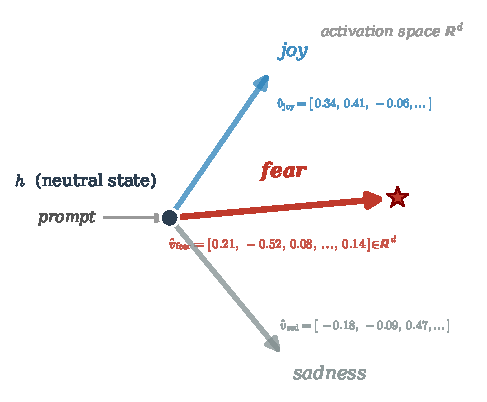
\includegraphics[width=0.85\columnwidth]{background_emotion_vector.pdf}
\caption{\textbf{Emotion vectors as directions in activation space (schematic).}
Conceptually, an emotion vector starts from a neutral model state~$h$.
A prompt that evokes a given emotion, such as fear, pushes the residual
stream toward a direction~$\hat{v}_{\text{fear}}$, encoded here with its
representative $d$-dimensional coordinates.
This direction behaves like a commuter who takes the same route to work
every day: the attitude, direction, and flow stay the same each time.
Across thousands of different prompts that express the same emotion in
different words, the model converges on this same direction through its
layers, and it produces its output by moving along that direction.
After \citet{sofroniew2026emotion}, who call this an emotion vector; we
reuse the geometry, not the construct.}
\label{fig:emotion_vector}
\end{figure}

\paragraph{From Emotions to Hiring.}
Nothing in this read-and-steer recipe is specific to emotion.
Any construct that is linearly encoded in the residual stream should, in
principle, be extractable by the same mean-difference procedure and
testable by the same steering intervention, whether that construct is an
emotional state or a dimension of social perception.
Hiring is a domain where such a construct would matter immediately:
behavioral audits have already documented that large language models produce
uneven callback recommendations across demographic groups
\citep{an2024llm, gaebler2024auditing}, yet none of that work locates the
representation inside the model that might be doing the work.
We therefore ask whether a social-perception construct known to predict
human callback outcomes is encoded the same way emotion concepts are, and
whether steering it changes a model's own callback recommendations.
The next section describes how we chose that construct and built the
materials needed to test it.

% ─────────────────────────────────────────────────────────────────────────────
\section*{Adapting the Method to Hiring}
% ─────────────────────────────────────────────────────────────────────────────

\paragraph{Why Warmth and Competence.}
The Stereotype Content Model proposes that social perception organizes along
two fundamental axes: warmth, capturing perceived intentions and
trustworthiness, and competence, capturing perceived ability and
effectiveness \citep{fiske2002model}.
Evidence across cultural contexts suggests that warmth and competence are
recurring dimensions of both interpersonal impressions and perceptions of
social groups \citep{fiske2007universal, cuddy2008warmth}.
Warmth and competence therefore give us two well-established, independently
motivated axes to search for inside a language model, rather than an
ad hoc pair invented for this study.

\paragraph{The Link to Hiring.}
\citet{gallo2024warmth} provide the empirical bridge that connects these two
axes to real labor-market outcomes.
Their released ratings data contain 24,220 warmth and competence judgments
from 787 raters covering 282 applicant first names drawn from ten source
studies.
For the eight name-based correspondence studies with usable callback data,
a more favorable first principal component combining warmth and competence
was moderately associated with higher callback rates on average.
The effect nevertheless varied substantially across studies, and its
prediction interval included negative relationships.
These findings provide a direct, quantitative connection between the
social-perception dimensions we probe and measured labor-market outcomes,
while showing that the relationship is not uniform.
Behavioral audits of LLMs have separately documented name-driven callback
disparities \citep{an2024llm, an_measuring_2025, gaebler2024auditing}.
To our knowledge, these studies have not tested whether internal warmth and
competence representations carry that signal.
We use the dataset released by Gallo et al. in two ways: as an external
validity check on our probes, and as the reference point against which
model-level disparities are compared.

\paragraph{Concept Stories Without Identity.}
Probing warmth and competence directly from hiring prompts would confound
the social-perception dimensions with the hiring decision itself, so the
direction vectors have to come from a separate set of materials.
We generated 200 short concept stories, evenly split across four conditions
(high warmth, low warmth, high competence, low competence), each built
around an everyday situation rather than a workplace scenario.
Every protagonist in these stories is nameless and gender-neutral, referred
to only as ``they.''
This design was not a default choice: pilot work showed that
LLM-generated concept stories without this constraint systematically
assigned male, Anglo-named protagonists to the low-warmth and
low-competence conditions, which would have baked demographic expectations
into the direction vectors before any hiring evaluation even began.
Removing names and gender from the stories forces each story's activation
to be driven by depicted behavior alone, keeping the concept vectors free of
the demographic signal we later test for.

\paragraph{Applicant Names.}
The hiring evaluation itself draws on a separate stimulus set: the 282
applicant first names from \citet{gallo2024warmth}, each inserted into an
otherwise identical, fixed job application so that the name is the only
signal that varies across trials.
Of these 282 names, 149 also appear in the published per-name callback
dataset from the same source and carry US race and gender labels; this
subset forms the benchmark comparison for demographic disparity.
The full set of 282 is used for the probe-versus-human alignment check,
since every name carries crowdsourced warmth and competence ratings even
when published callback data are unavailable.

% ─────────────────────────────────────────────────────────────────────────────
\section*{Methods}
% ─────────────────────────────────────────────────────────────────────────────

\paragraph{Story Preparation.}
We generated 200 short narratives (about 90--150 words each), split evenly
across four conditions: high warmth, low warmth, high competence, and low
competence (50 stories per condition).
Stories were written around 50 everyday topics spanning ten domains
(workplace, learning, community, sport, travel, and others), with each topic
appearing once per condition so that situational vocabulary stays balanced
between the high and low poles.
Every story uses a nameless, gender-neutral protagonist (``they''), for the
reasons given above.
Stories were generated by a large language model and checked automatically
for forbidden-vocabulary violations, length balance across conditions, and
demographic neutrality.
This design raises a circularity concern, since the same family of models
that wrote the stories is later probed for the concepts those stories
express; we return to this point in the Limitations.

\paragraph{Building the Warmth and Competence Vectors.}
We used TransformerLens \citep{nanda2022transformerlens} to extract
residual-stream activations from nine open-weights instruction-tuned models
spanning three model families and two version generations each for Gemma and
Qwen: Gemma-3-12B-it and Gemma-3-27B-it \citep{gemmateam2025gemma3},
Gemma-4-12B, Gemma-4-26B-A4B, and Gemma-4-31B; Qwen3-14B
\citep{qwen2025qwen3}, Qwen3.6-27B, and Qwen3.6-35B-A3B; and
Llama-3.1-8B-Instruct \citep{grattafiori2024llama3}.
For each model we captured the residual-stream state at the layer
corresponding to about 65 percent of model depth, chosen from a full layer
sweep of Cohen's~$d$ values (\autoref{tab:models} reports the exact probe
layer, model width, and mean residual-stream norm for each model).
For each story, activations were mean-pooled across token positions from
position~50 onward, skipping the prompt prefix, giving one
$d_\mathrm{model}$-dimensional vector per story.
High- and low-condition stories cluster in distinct regions of this space
(\autoref{fig:concept_geometry}), and the warmth and competence direction
vectors are simply the mean difference between the two clusters,
$v_W = \bar{x}_\mathrm{high\,warmth} - \bar{x}_\mathrm{low\,warmth}$ and
$v_C = \bar{x}_\mathrm{high\,comp.} - \bar{x}_\mathrm{low\,comp.}$.
All nine models were run under identical conditions (same stories, same
pooling rule, same seed 20260527) so that results can be compared across
architectures.
Every step described in this section, vector building, probe validation,
concept- and hiring-level steering, and the hiring evaluation and disparity
analysis below, was applied identically to all nine models; complete
per-model results for the full suite appear in the Supplementary appendix
tables, and \autoref{tab:models} reports parameters for all nine.

\begin{table}[t]
\centering
\small
\caption{%
  Model parameters and probe extraction settings for all nine checkpoints.
  Probe layer is given as selected/total layers.
  $\bar{\|h\|}$ is the mean residual-stream norm at the probe layer, which sets
  the scale of steering interventions; the difference across models spans
  several orders of magnitude, so raw-strength comparisons are not meaningful
  without normalization.
}
\label{tab:models}
\begin{tabular}{lcccc}
\toprule
Model & $d_\mathrm{model}$ & Probe layer & $\bar{\|h\|}$ \\
\midrule
Gemma-3-12B-it          & 3840 & 31/48 & 79{,}722 \\
Gemma-3-27B-it          & 5376 & 40/62 & 61{,}576 \\
Gemma-4-12B             & 3840 & 31/48 & 97.8     \\
Gemma-4-26B-A4B         & 2816 & 19/30 & 68.4     \\
Gemma-4-31B             & 5376 & 39/60 & 188.5    \\
\addlinespace
Qwen3-14B               & 5120 & 26/40 & 206.6    \\
Qwen3.6-27B             & 5120 & 42/64 & 71.9     \\
Qwen3.6-35B-A3B         & 2048 & 26/40 & 3.6      \\
\addlinespace
Llama-3.1-8B-Instruct   & 4096 & 20/32 & 11.4     \\
\bottomrule
\end{tabular}
\end{table}

We check that each direction is a genuine, generalizable signal rather than
an artifact of the specific stories used to build it, using five
complementary checks: (i)~5-fold cross-validated accuracy, where a logistic
regression classifier is trained on full residual-stream representations and
scored on held-out folds; (ii)~topic-holdout accuracy, a stricter variant
using GroupKFold in which all stories from a given topic sit in the same
fold, so the probe is tested on entirely unseen situations rather than
unseen phrasings of familiar ones; (iii)~Cohen's~$d$, the standardized mean
difference between high- and low-condition projections onto the direction,
compared against an empirical null of 1,000 random unit vectors;
(iv)~split-half cosine stability, where each condition's 50 stories are
randomly split into halves of 25 and the cosine between the two resulting
directions is reported; and (v)~cross-axis classification, which tests
whether the warmth direction predicts competence labels and vice versa, to
quantify shared evaluative content between the two axes.
We also compute per-story Spearman rank correlations across model pairs to
test whether the models converge on a shared cross-architecture construct
rather than independent, unrelated ones.
A neutral-corpus PCA denoising procedure separates this shared evaluative
content from the target concepts; the Supplementary Materials (PCA
Denoising) describe the full procedure as a robustness check.

\paragraph{Steering the Concept Vectors.}
A direction that merely separates high- and low-condition activations does
not yet show that the model relies on it; to test that, we apply activation
steering \citep{turner2023activation} via TransformerLens hooks at the probe
layer (\autoref{fig:concept_geometry}).
Steering strength is expressed relative to the mean residual-stream norm at
that layer, so that interventions are comparable across models whose
activation scales differ by orders of magnitude (see $\bar{\|h\|}$ in
\autoref{tab:models}).
At the concept level, the model answers ``Is the protagonist high in
warmth/competence? Answer only Yes or No'' on held-out topics (40 for
training, 10 for testing, split by topic index), while we push the
residual stream along a local grid of $\alpha \in
\{-0.10,\,-0.05,\,0,\,+0.05,\,+0.10\}$ times the mean norm.
The outcome is the next-token logit margin $\Delta =
\mathrm{logit}(\text{Yes}) - \mathrm{logit}(\text{No})$.
We compare six candidate directions at this stage: the dense target
direction, a decoded Gemma Scope~2 SAE direction
\citep{deepmind2025gemmascope2}, an axis-specific component, a component
shared between the two axes, the opposing concept axis, and a random
orthogonal control, since a real effect should be specific to the target
direction and absent for an unrelated one.
Uncertainty throughout is estimated by paired topic bootstrap resampling.

\begin{figure}[t]
\centering
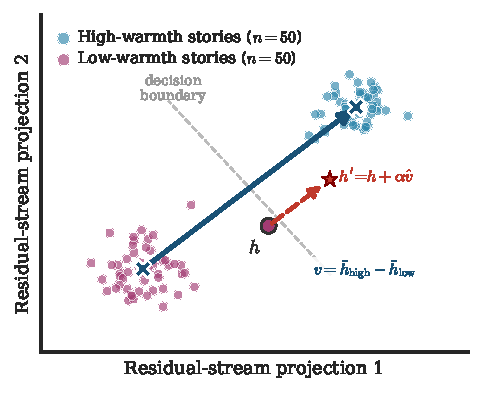
\includegraphics[width=0.85\columnwidth]{background_concept_geometry.pdf}
\caption{\textbf{Residual-stream concept geometry (schematic).}
Low-warmth and high-warmth stories occupy different regions of this space,
and the mean-difference direction
$v = \bar{h}_{\mathrm{high}} - \bar{h}_{\mathrm{low}}$ (blue arrow) is what
separates them.
Steering acts like grabbing the wheel of a car that is already driving down
one street and turning it until the car crosses onto the next street over:
the red dashed arrow, $h' = h + \alpha\,\hat{v}$, shows this same kind of
forced redirection, pushing a story's representation from the low-warmth
region, across the decision boundary, into the high-warmth region.
Concretely, this is done by adding a scaled copy of that same high-warmth
direction to the story's current representation.
Illustrative synthetic activations, not measured data.}
\label{fig:concept_geometry}
\end{figure}

\paragraph{Steering Hiring Decisions.}
The hiring prompt pairs each of the 282 applicant first names from
\citet{gallo2024warmth} with an otherwise identical, fixed
administrative-assistant application (same education, experience, and
skills in every trial), so the name is the only signal that varies.
The model answers ``would you recommend calling this candidate back for an
interview? Answer with a single word: Yes or No,'' and the outcome is the
\textit{callback margin}, the logit difference
$\mathrm{logit}(\text{Yes}) - \mathrm{logit}(\text{No})$.
Race and gender labels are never shown to the model; they are assigned
afterward from the \citet{gallo2024warmth} coding, mirroring the design of
human correspondence studies \citep{bertrand2004emily}.
We then apply the same steering hooks used at the concept level while the
model processes these resume-evaluation prompts over a 60-name subset of
the applicant roster, using a broad sweep at $\alpha \in
\{\pm 0.25,\,\pm 0.50\}$ and a local-regime follow-up at
$\{\pm 0.05,\,\pm 0.10\}$ for the two Gemma models, so that a push on the
warmth or competence direction can be traced directly to a shift in the
callback margin.

\paragraph{Names, Human Ratings, and Disparity.}
Independently of the hiring prompt, each applicant name is embedded in a
neutral carrier sentence, and its residual-stream activation is projected
onto the warmth and competence directions to yield a per-name probe score.
We compare these scores against the aggregated human ratings behind them
(24{,}220 rater judgments from 787 raters across ten source studies) using
Spearman rank correlation, which tells us whether the model's internal
sense of a name's warmth or competence lines up with how people actually
perceive that name.
Group-level callback disparities are then computed as differences in mean
callback margin between name groups (race: 47 Black-signaling versus 180
White-signaling names; gender: 154 female versus 115 male), standardized by
the within-model standard deviation of the callback margin so that models
with different logit scales can be compared on equal footing.
Human reference gaps come from the published per-name callback rates,
aggregated over the 149 names that match the benchmark on first name.
Finally, we test whether the internal warmth and competence representations
actually carry the name-group signal into the callback decision, using
bootstrap mediation along the path name group~$\to$ probe score~$\to$
callback margin (5{,}000 resamples, seed 20260527, $n = 269$ names with
complete data, race subset $n = 227$), reporting indirect effects with 95\%
confidence intervals for all sixteen model-by-grouping-by-probe
combinations.

% ─────────────────────────────────────────────────────────────────────────────
\section*{Results}
% ─────────────────────────────────────────────────────────────────────────────
% Results — to be redesigned collaboratively (next round).
% Parked figures/tables below: environments and labels are kept in place so
% existing \autoref pointers elsewhere in the document (including the
% Supplementary) keep resolving, and so the redesign can reposition or
% recaption them without regenerating any plots.

% parked figures for redesign
\begin{figure*}[t]
\centering

\includegraphics[width=\textwidth]{paper_figure1_axis_arrows.pdf}
\caption{\textbf{Warmth and competence directions share model-dependent geometry.}
Each panel projects the same 200 synthetic stories onto raw dense probe-layer
directions in an oblique basis. The arrow angle equals
$\arccos[\cos(v_W,v_C)]$, so smaller angles indicate stronger geometric
alignment. All panels use model-internal z-scores, shared axis limits, and
equal x/y scaling.}
\label{fig:paper_figure1_axis_arrows}
\end{figure*}

\begin{figure*}[t]
\centering

\includegraphics[width=\textwidth]{paper_figure2_layer_emergence.pdf}
\caption{\textbf{Warmth and competence directions emerge robustly across depth.}
Layer-wise Cohen's~$d$ across nine open-weights models. The dotted vertical
line marks the fixed probe-layer fraction of 0.66.}
\label{fig:paper_figure2_layer_emergence}
\end{figure*}

\begin{figure*}[t]
\centering

\includegraphics[width=\textwidth]{fig14_dense_steering_normalized.pdf}
\caption{\textbf{Normalized concept-level steerability varies across nine
checkpoints.} Each curve shows the additive target-direction change in the
held-out Yes-versus-No concept margin divided by the baseline high-versus-low
margin gap for the same model and axis. Parentheses in the legend report the maximum
positive steering coefficient, $\alpha=+0.10$, expressed relative to the mean
residual norm. Normalization reduces raw logit-scale differences but does not
establish direction specificity; calibrated random and cross-axis controls are
interpreted in the text.}
\label{fig:fig14_dense_steering_normalized}
\end{figure*}

% Generated by src/build_paper_probe_tables.py.
% Source: results/logs/hiring_probe_vs_human_<label>.json, data/processed/<vectors_subdir>/meta.json.
% table* spans both columns of the twocolumn body (Section 1 of
% Ulu_Lastra.tex); a single-column table with \resizebox{\textwidth}
% would overflow into the adjacent column.
\begin{table*}[t]
\centering
\small
\setlength{\tabcolsep}{4pt}
\resizebox{\textwidth}{!}{%
\begin{tabular}{@{}lccccc@{}}
\toprule
Model & Probe layer (frac) & $\rho$(warmth, human) & $\rho$(competence, human) & $\rho$(callback, warmth) & $\rho$(callback, competence) \\
\midrule
Gemma-3-12B & 31 (0.65) & +0.357*** & +0.237*** & +0.150* & +0.149* \\
Gemma-3-27B & 40 (0.65) & +0.388*** & +0.271*** & -0.160** & -0.156** \\
Llama-3.1-8B & 20 (0.62) & -0.287*** & -0.058 n.s. & +0.092 n.s. & +0.053 n.s. \\
Gemma-4-12B & 31 (0.65) & +0.009 n.s. & +0.216*** & -0.110 n.s. & -0.124* \\
Gemma-4-26B-A4B & 19 (0.63) & -0.190** & -0.044 n.s. & +0.510*** & +0.373*** \\
Gemma-4-31B & 39 (0.65) & +0.254*** & +0.290*** & +0.024 n.s. & +0.337*** \\
Qwen3-14B & 26 (0.65) & -0.178** & +0.466*** & +0.195** & +0.426*** \\
Qwen3.6-27B & 42 (0.66) & +0.192** & +0.247*** & +0.302*** & +0.220*** \\
Qwen3.6-35B-A3B & 26 (0.65) & +0.206*** & +0.130* & +0.344*** & +0.197*** \\
\bottomrule
\end{tabular}%
}
\caption{\textbf{Name-level correlation between probed warmth/competence and human ratings.} For each of the 282 rated applicant names, the model's residual-stream activation at the probe layer is projected onto the warmth and competence direction vectors. ``Probe layer'' gives the selected layer index and its resolved fraction of total depth (targeted $\mathrm{probe\_layer\_frac}=0.66$; the reported fraction is the integer-rounded layer divided by model depth). Warmth/competence columns correlate the probe projection with human warmth/competence ratings; callback columns correlate the probe projection with the model's own unsteered callback margin. All correlations are Spearman $\rho$. $^{*}p<.05$, $^{**}p<.01$, $^{***}p<.001$, n.s. not significant.}
\label{tab:probe_human}
\end{table*}


\begin{figure*}[t]
\centering
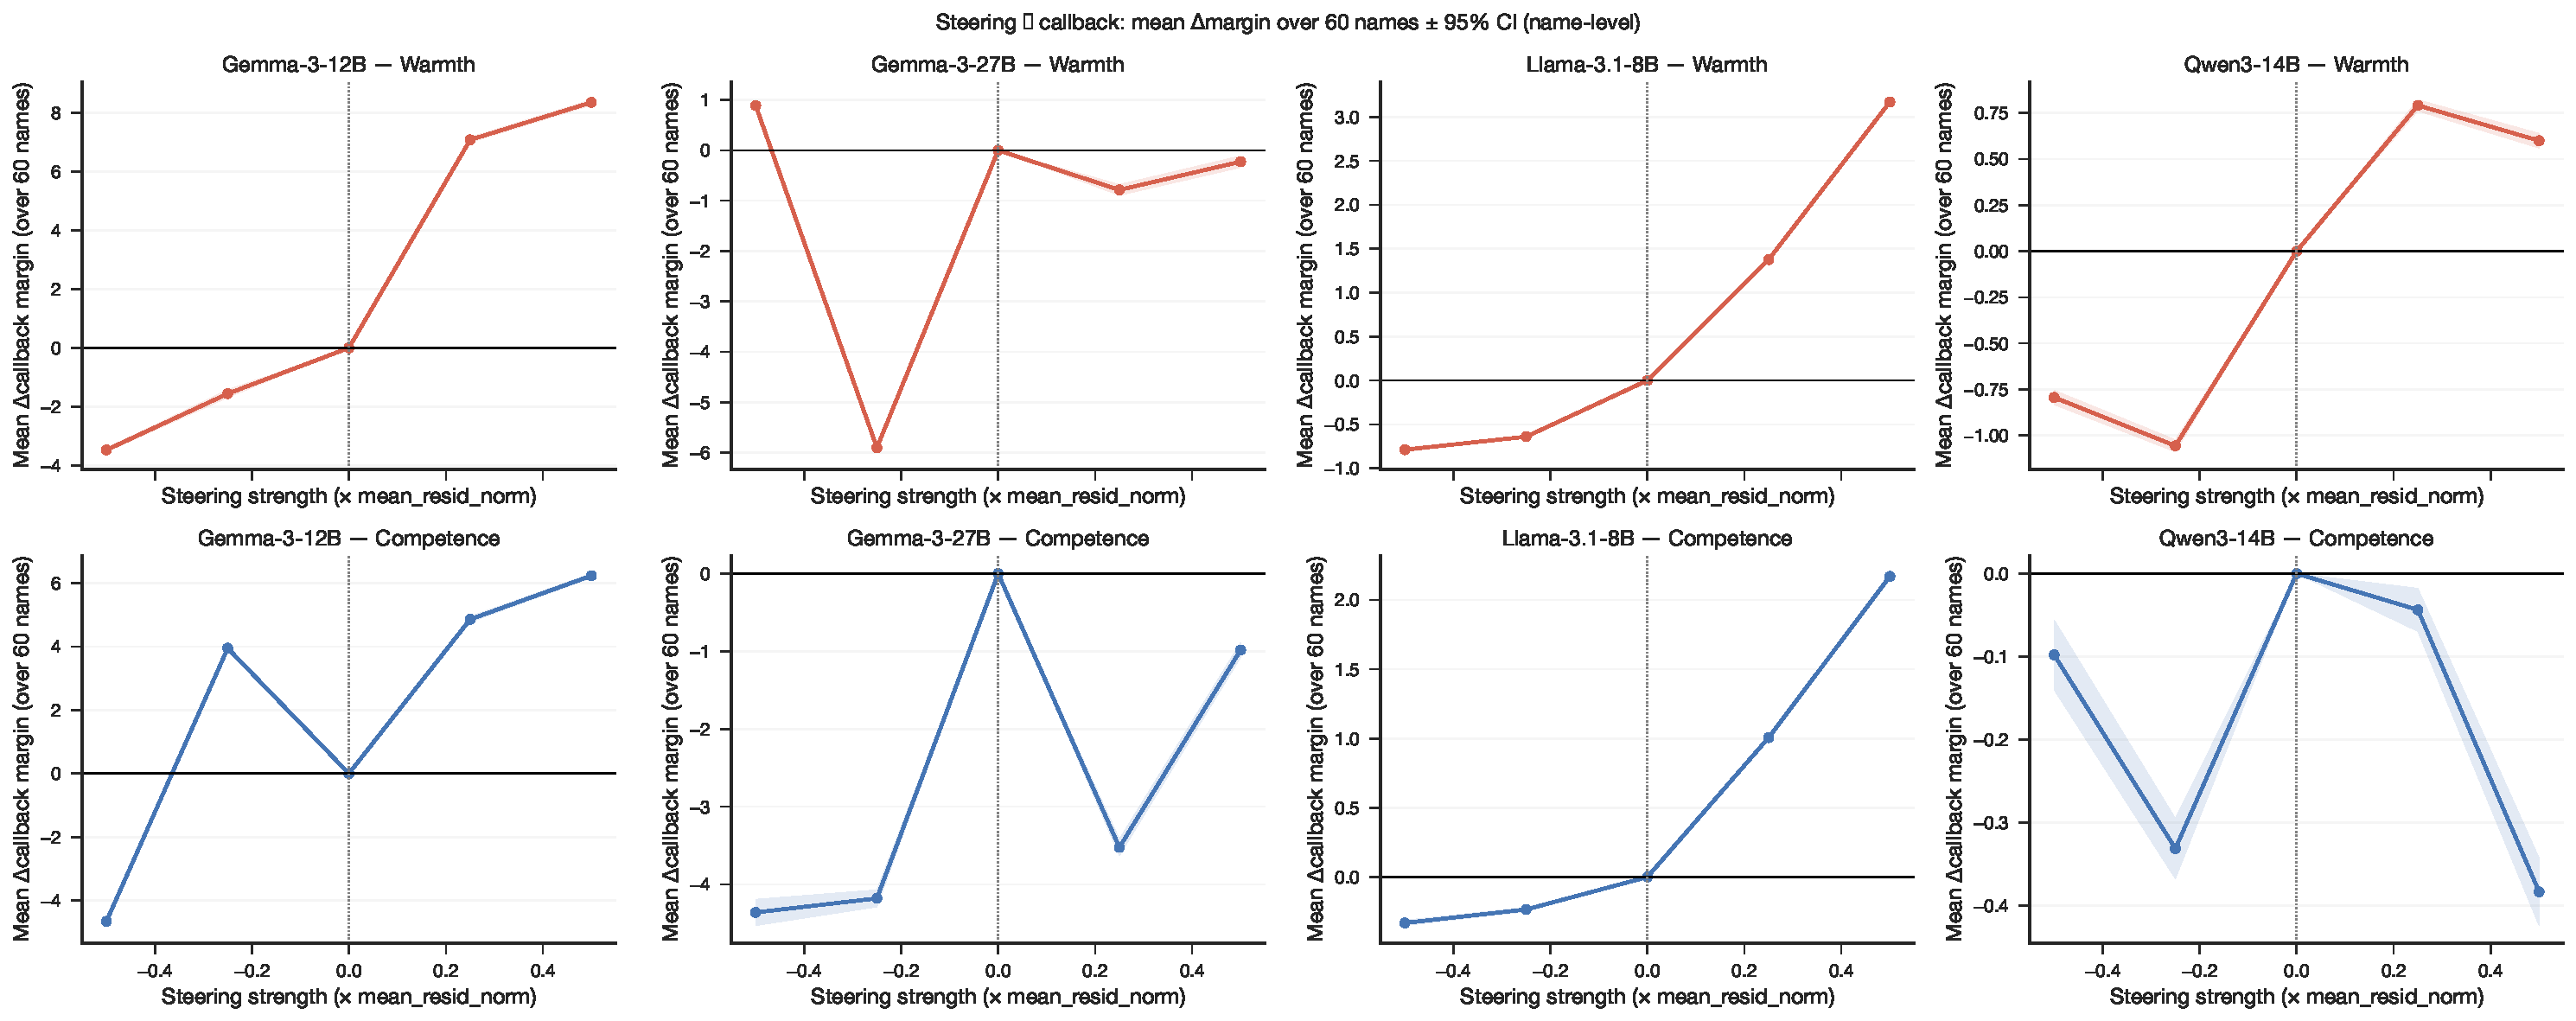
\includegraphics[width=\textwidth]{fig17_hiring_steering_callback.pdf}
\caption{\textbf{Activation steering shifts hiring callback recommendations.}
Callback-margin responses to warmth and competence steering in the hiring
evaluation setting.}
\label{fig:fig17_hiring_steering_callback}
\end{figure*}

\begin{figure*}[t]
\centering
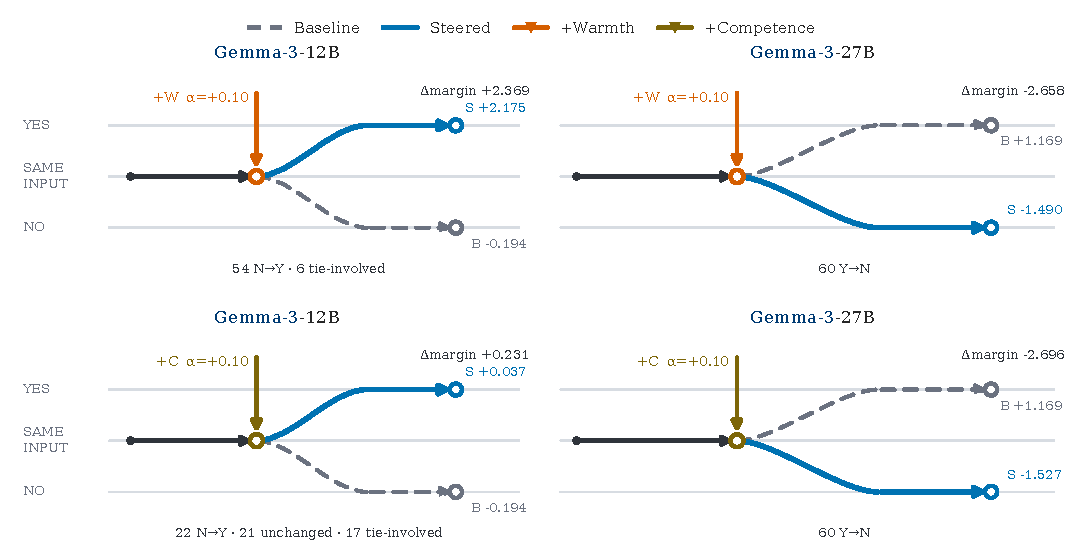
\includegraphics[width=\textwidth]{paper_figure4_hiring_bidirectional_examples.pdf}
\caption{\textbf{Matched examples show that positive concept steering can move
callback decisions in either direction.}
Rows show warmth and competence; columns compare Gemma-3-12B, whose mean
decision moves from No to Yes, with Gemma-3-27B, whose mean decision moves from
Yes to No. All panels use the same 60 applications and $\alpha=+0.10$.
Gray dashed paths show baseline outcomes, blue paths show steered outcomes, and
bottom annotations summarize individual-name transitions. The panels were
selected to display both transition directions under matched conditions, not to
estimate their prevalence. Endpoint margins, strengths, and transition counts
are empirical; connector geometry is schematic. Complete results for all nine
models and both axes appear in \autoref{tab:hiring_transition_census}.}
\label{fig:hiring_bidirectional_examples}
\end{figure*}

\begin{figure*}[t]
\centering

\includegraphics[width=\textwidth]{fig13_dense_steering_doseresponse.pdf}
\caption{\textbf{Dense steering dose-response across models.}
Concept-level dose-response curves for warmth and competence directions.}
\label{fig:fig13_dense_steering_doseresponse}
\end{figure*}

\begin{figure*}[t]
\centering
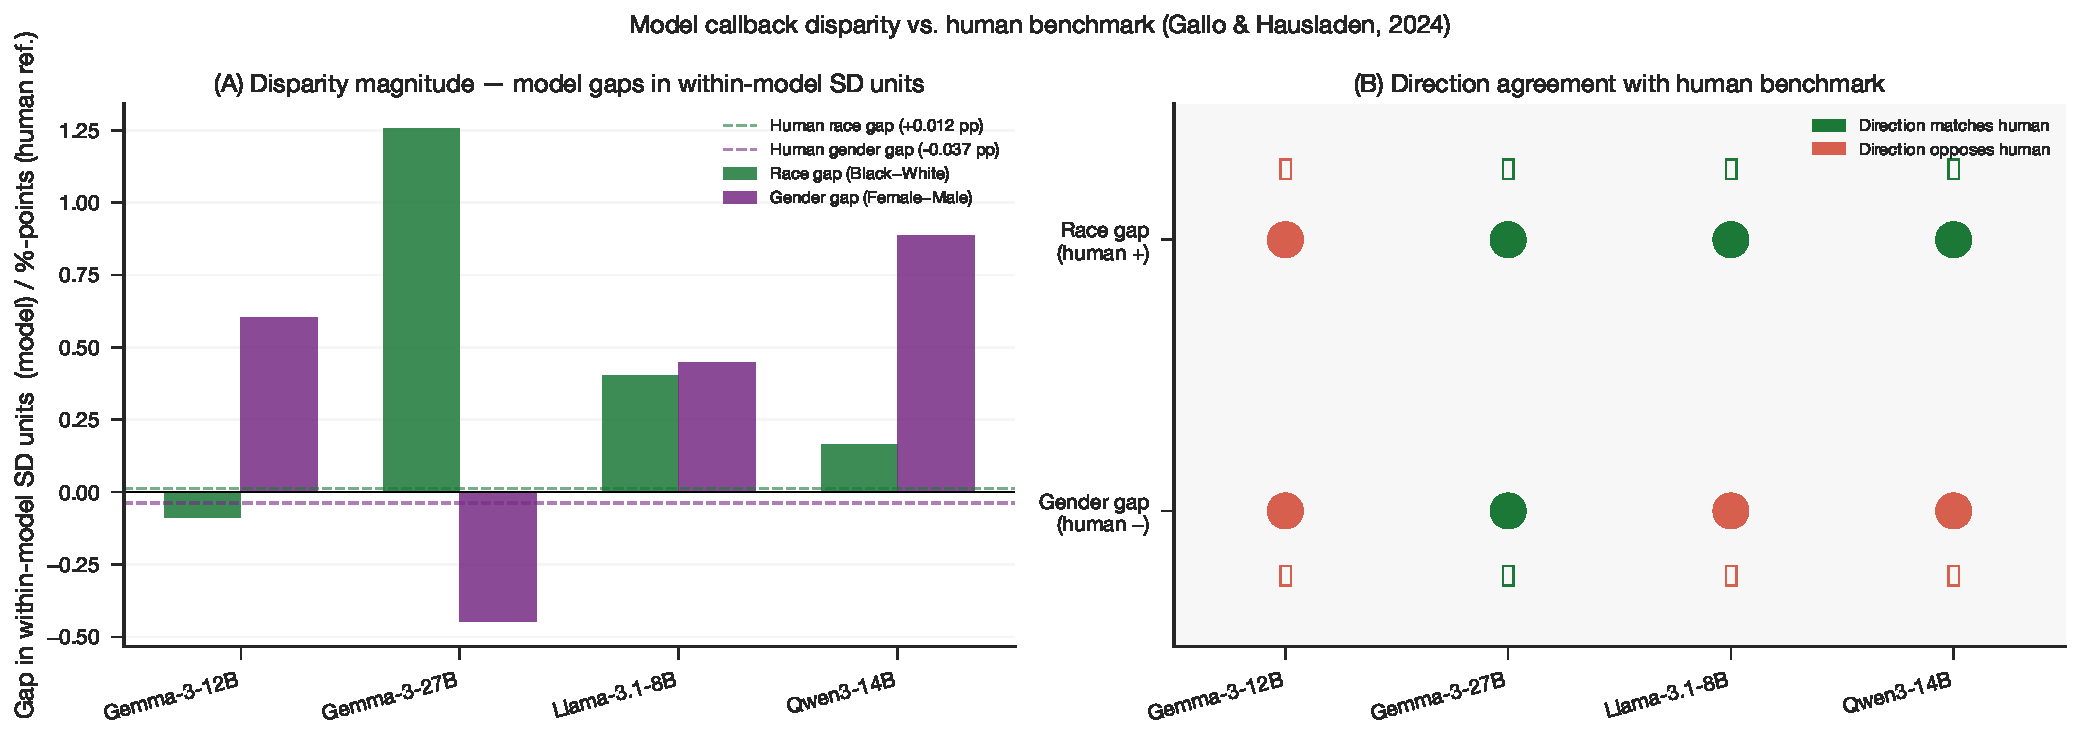
\includegraphics[width=\textwidth]{fig18_hiring_disparity.pdf}
\caption{\textbf{Model callback disparities relative to the human benchmark.}
Race and gender callback-margin gaps for the model evaluations compared with
the correspondence-study benchmark.}
\label{fig:fig18_hiring_disparity}
\end{figure*}

\begin{figure*}[t]
\centering
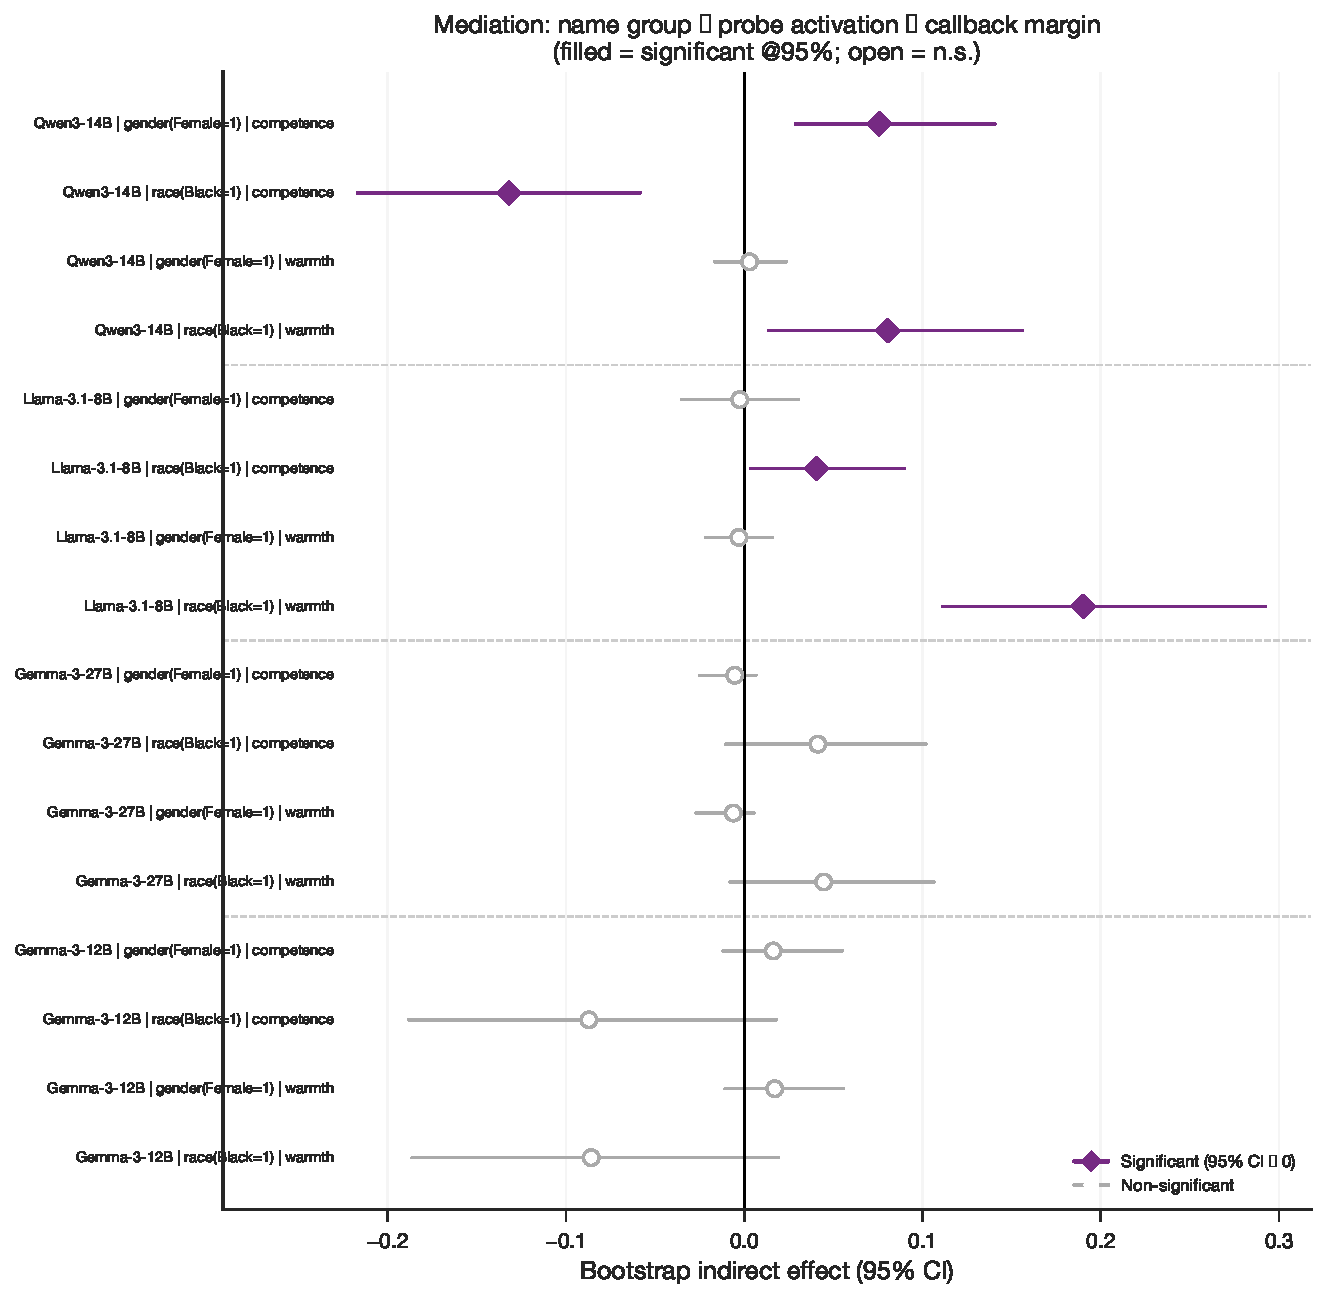
\includegraphics[width=\textwidth]{fig19_hiring_mediation_forest.pdf}
\caption{\textbf{Bootstrap mediation of name-group callback disparities
through warmth and competence probe scores.}
Indirect effects with 95\% confidence intervals for the pathway name group
$\to$ probe score $\to$ callback margin; filled markers indicate intervals
that exclude zero.}
\label{fig:fig19_hiring_mediation_forest}
\end{figure*}

% ─────────────────────────────────────────────────────────────────────────────
\section*{Discussion and Conclusion}
% ─────────────────────────────────────────────────────────────────────────────

That large language models trained on human-generated text would encode
warmth and competence as internally recoverable representations is,
in one sense, not surprising: these models distil patterns from the
same texts in which warmth and competence shape social perception.
What the present results establish empirically is that this encoding is
linear, geometrically stable, causally functional at the concept level,
and shared across architecturally distinct models from independent
laboratories.
Each of these properties matters: linearity makes the representation
accessible to lightweight probes and steering interventions; causal
functionality means the representation participates in explicit
judgements about warmth and competence; and cross-architecture
convergence suggests the finding reflects a property of training data
and the objectives of language modelling rather than a quirk of any
single design.

The scale comparison between Gemma-3-12B and Gemma-3-27B complicates
this picture in an instructive way.
Both models encode warmth and competence with comparable precision, and
the 27B model's probe scores correlate slightly more strongly with human
warmth and competence ratings.
Yet the causal chain from concept representation to hiring decision differs
sharply between them.
At 12B, increasing the warmth representation produces a large, approximately
linear increase in callback inclination (up to $+2.37$ logit units at
$\alpha = +0.10$).
At 27B, the equivalent intervention produces a modest positive shift at low
strength ($+1.97$ at $\alpha = +0.05$) that collapses to a large negative
shift at slightly higher strength ($-2.66$ at $\alpha = +0.10$).
This non-monotone response is not saturation: the 27B baseline already
sits at $P(\text{Yes}) = 0.76$, leaving room for upward movement, and
the response is a sign reversal rather than a plateau.
A more plausible account is that the 27B decision layer is organised by
multiple interacting representations; the concept direction, when
amplified beyond a narrow window, begins to interfere with those
interactions rather than reinforcing them.

A related puzzle emerges from the cross-model steerability analysis.
Among the models with local-regime mediation estimates, Gemma-3-12B has
the largest normalized warmth steerability ($0.236$), yet it shows no
significant hiring-level mediation path. Llama-3.1-8B has the smallest
value within that subset ($0.029$) and shows the strongest hiring-level
indirect effect (bootstrap IE $= +0.190$).
This steerability paradox illustrates that the capacity to shift a
model's representations via linear probing does not imply that those
representations causally govern the downstream decision.
Models in which representations are most cleanly isolable may be
precisely those in which decision processes operate through parallel
mechanisms that bypass the steering target.

The warmth anti-alignment observed in Llama-3.1-8B and Qwen3-14B adds
a further layer of complexity.
Despite high cross-model story agreement (per-story Spearman $\rho
\approx 0.76$--$0.77$ between Gemma and each of the other models),
the direction that Llama and Qwen organise as ``high warmth'' in
activation space is negatively correlated with human warmth ratings
($\rho = -0.300$ and $-0.193$ respectively).
The models converge on the same relative ordering of stories yet that
shared ordering is inverted relative to the human scale.
We interpret this as evidence that instruction tuning has restructured
the warmth axis in these architectures: reinforcement learning from
human feedback may have adjusted representations associated with
stereotypically warm social groups in a direction that happens to
invert the relationship to the original pretraining warmth axis.

The demographic disparity results at Gemma-3-27B illustrate the
practical consequence of this representational reorganisation.
The model strongly advantages Black-signalling names relative to
White-signalling names ($+1.18$ SD), directly reversing the classical
correspondence-study finding.
The gender gap direction, by contrast, reproduces the human pattern.
The asymmetry between race and gender suggests that instruction tuning
has applied differential corrections to different demographic axes,
producing a model that is not more equitable overall but differently
inequitable: the racial hierarchy is reversed rather than eliminated,
and at substantially larger magnitude than the original human disparity.
This finding points to a fundamental limitation of outcome-level bias
mitigation: correcting behavioral outputs without understanding the
representational substrate can shift rather than remove the underlying
imbalance.

Together, the results suggest that LLMs have internalised a structure of
social perception broadly analogous to the SCM, emerging from training on
human-generated text rather than through any explicit design choice.
The connection from that internal structure to actual hiring decisions is
not, however, simple or consistent across models.
This finding points to a methodological implication for bias auditing:
probing internal representations and measuring output disparities are
complementary but not interchangeable, and a model that performs well on
one measure may not perform well on the other.
It also opens a path to addressing the problem at the source by
intervening on the representation rather than filtering outputs after
the fact, and provides a methodological template for connecting the
computational tools of mechanistic interpretability to the empirical
tradition of correspondence studies in the social sciences.

\paragraph{Limitations.}
The concept story corpus was generated by a large language model,
raising concerns about circularity in a study that probes language
model representations.
We note, however, that the generating model (Claude, Anthropic) and
the probed models (Gemma, Qwen, Llama) come from different
organisations and architectures, so the warmth/competence contrasts
are not trivially reproduced by a shared generator.
Nevertheless, the possibility that AI-generated stimuli share stylistic
properties that inflate probe accuracy across model families cannot be
fully excluded; replication with human-authored or template-based
stimuli is desirable.
The corpus covers 50 topics; broader topic coverage and larger
per-condition samples would further test how far the directions
generalize.
The probe-to-human validation correlations are moderate (warmth
$\rho = +0.366$ and $+0.396$ for 12B and 27B; competence $\rho = +0.239$
and $+0.272$), indicating that the model's internal probes capture a
component of human social perception rather than replicating it
faithfully.
The warmth anti-alignment in Llama-3.1-8B ($\rho = -0.300$) and
Qwen3-14B ($\rho = -0.193$) means that for these models the mean-difference
direction captures a construct that is systematically inverted relative to
the human warmth scale; results for these models should be interpreted
with this inversion in mind.
The probe layer for every model is fixed by a single heuristic,
$\mathrm{probe\_layer\_frac} = 0.66$, rather than selected for maximum
warmth/competence separability. A full-depth layer sweep on the training
story corpus shows that this heuristic layer rarely coincides with the
layer of peak separability: at Gemma-3-12B the selected layer reaches a
warmth Cohen's $d$ of 2.68, while the best-separated layer in the same
sweep reaches 6.27; Gemma-3-27B (2.95 versus 5.10) and Gemma-4-31B (7.56
versus 11.49) show comparable gaps. This mismatch does not fully explain
the weak or inverted name-level correlations reported above. Gemma-4-12B
already reaches a high separability score at its selected layer
($d = 8.46$), yet the resulting warmth probe fails to correlate with human
name ratings ($\rho = +0.020$, n.s.). Story-level separability, which
guides layer selection, therefore does not guarantee that the resulting
direction generalises to bare applicant names, a case the training stories
never present. Whether averaging or weighting probe projections across the
several most separable layers would recover a stronger name-level signal
than the single fixed layer is a question we leave open.
The causal warmth steering effect at the hiring level is positive and
strong at 12B but non-monotone and fragile at 27B, so the causal claim
does not generalise across scale without qualification.
Callback margins are quantised to a 0.125-unit grid due to bf16 precision
in the model's output logits; this quantisation is inherent to bf16
inference and is not resolved by float32 subtraction.
We attempted a partial fix by casting the Yes/No logits to float32 before
subtracting them, which removes rounding in the subtraction step itself,
but the two operands are already bf16-quantised by the time they reach
that subtraction, so the 0.125 grid persists regardless. A complete fix
would require running inference itself in float32, which roughly doubles
GPU memory usage and is likely infeasible for the 27B checkpoint on the
available cluster hardware; we did not attempt it.
At Gemma-3-12B the callback margin standard deviation is 0.14 with only
seven unique values, making group-level disparity estimates at 12B
unreliable and the 12B R4 results should not be cited as empirical
findings. Llama-3.1-8B shows a comparably narrow spread (SD $= 0.12$,
12 unique values), so its group-level gaps should be read with the same
caution.
At Gemma-3-27B the larger variance (SD $= 0.41$, 18 unique values)
makes group gaps of approximately 0.5 SD detectable, but the grid
structure introduces discrete steps in all reported gap magnitudes.
Qwen3-14B (SD $= 0.35$, 17 unique values) falls in the same usable range
as 27B.
The sixteen mediation tests are presented uncorrected for multiple
comparisons; only the Llama race--warmth indirect effect survives a
Bonferroni-corrected threshold, and the smaller significant paths should
be treated as suggestive rather than confirmed.
The hiring prompt is simplified relative to real-world screening contexts
(single role, fixed qualifications), and results may differ under richer
evaluation settings or different job types.
Finally, the architectural source of the elevated warmth/competence
vector cosine observed in Gemma-3 relative to Qwen3 and Llama-3.1
across all network depths remains an open question.

\paragraph{Future Work.}
The immediate next step is expanding the hiring stimuli to additional
job roles to test whether results generalise beyond administrative
assistant.
The SAE decomposition performed here on Gemma-3 can be extended to
Llama-3.1 using the Llama Scope sparse autoencoders \citep{lindsey2025llama},
enabling a model-family comparison at the feature level.
Validating the concept probes against a human-authored warmth/competence
dataset would address the circularity concern associated with
AI-generated stimuli.
On the social-science side, extending the hiring stimuli beyond names to
category-level signals (age, disability, religion) would broaden the
scope of the benchmark comparison and test whether the representational
account generalises beyond race and gender.
Translating these findings into practical debiasing interventions and
evaluating their robustness to adversarial prompting is a natural next
step for applied work.

{
\small

\clearpage
\printbibliography
}



\clearpage
\begin{appendices}
\onecolumn
\setcounter{figure}{0}
\setcounter{table}{0}
\renewcommand{\thesection}{\Alph{section}}%
\renewcommand{\thesubsection}{\thesection.\arabic{subsection}}
\renewcommand\thefigure{S.\arabic{figure}}
\renewcommand\thetable{S.\arabic{table}}
\begin{center}
    \begin{minipage}{\textwidth}
        \centering
        \fontsize{16}{20}\selectfont
        Supplementary Materials
    \end{minipage}
\end{center}
\vspace{.5cm}

\section*{Details on Methods}
\label{apx:methods}

\subsection*{Compute and Hardware}

All experiments ran on two compute environments.
The SCCKN cluster (Universit\"at Konstanz) supplied NVIDIA RTX PRO 6000
Blackwell GPUs (96 GB VRAM), which ran the Gemma-3, Llama-3.1, and Qwen3
jobs (Gemma-3-12B, Gemma-3-27B, Llama-3.1-8B, Qwen3-14B) and most of the
extraction and steering jobs for the Gemma-4 and Qwen3.6 checkpoints.
Gemma-4-12B is a partial exception: its Stage 1 activations were first
extracted on an NVIDIA L40, and a later retry ran on an L40S instead.
A dedicated reproducibility audit on the exact L40 hardware class found
that both device classes agree on which layer peaks for warmth and
competence (layers 26 and 27, respectively), but differ non-negligibly at
some layers (maximum competence Cohen's~$d$ difference of 0.914, cosine
difference of 0.095).
The exact-L40 run, hardware-matched to the original Stage 1 extraction, is
the one reported throughout the main text.
Select calibrated-steering replications for the Gemma-4 and Qwen3.6
checkpoints (all three Gemma-4 models and both Qwen3.6 models) instead ran
on NVIDIA H100 GPUs at the Collective Computational Unit (CCU).
The authors acknowledge support by the local computing resources through
the core facility SCCKN.
The authors additionally acknowledge the Collective Computational Unit
(CCU) for providing H100 GPU access used in part of this work.

\subsection*{PCA Denoising}

The warmth and competence direction vectors share a substantial common
component that reflects general narrative valence: stories that portray a
protagonist positively (whether warmly or competently) occupy a similar
region of the residual stream, and the same holds for negatively valenced
stories.
To separate conceptual content from this shared evaluative polarity, we
follow the neutral-corpus denoising procedure of \citet{sofroniew2026emotion}.
We build a neutral corpus of 1,500 Wikipedia introduction paragraphs,
length-matched to the concept stories (90--200 words) and filtered to
exclude emotionally charged or violent content, and extract residual-stream
activations at the same layer and pooling rule used for the concept stories.
We then fit principal component analysis (PCA) on these neutral activations
and project out, from both direction vectors, the top components that
together explain at least 50 percent of neutral variance.
For Gemma-3-12B, the first principal component alone explains 56.1 percent
of neutral variance, and removing it lowers the cosine between the warmth
and competence vectors from 0.749 to 0.530.
For Gemma-3-27B, 43 components are needed to cross the 50 percent threshold
(50.2 percent explained), lowering the inter-axis cosine from 0.708 to 0.487.
The remaining post-denoising cosine, 0.53 and 0.49 respectively, is close to
the genuine warmth-competence correlation observed in human ratings
($r \approx 0.61$; \citealt{fiske2002model}), which suggests that the
residual overlap reflects real conceptual co-variation rather than a
failure of the denoising step.
The denoised vectors serve as a robustness check; the raw dense directions
define the primary cross-model causal comparisons and the callback-transition
census reported in the main text.

\section*{Additional Results}

\subsection*{Complete Positive-Steering Callback Transitions}

\autoref{tab:hiring_transition_census} reports every model-axis condition used
in the positive-endpoint comparison. The table is the complete result; the
matched panels in \autoref{fig:hiring_bidirectional_examples} are illustrative
examples selected under a common family, application set, and steering strength.
Gemma-3-12B, Gemma-3-27B, and the Qwen3.6 and Gemma-4 checkpoints use
$\alpha=+0.10$. Llama-3.1-8B and Qwen3-14B use their available broad-regime
endpoint of $\alpha=+0.50$, so raw effect sizes should not be compared directly
across all rows.

Positive steering crosses the mean decision boundary in both directions among
the Gemma-3 models and from No to Yes for Llama-3.1-8B. The other six models
remain in the Yes category for every name, even when the mean margin decreases.
This pattern reflects two distinct mechanisms. First, a concept direction
constructed from high-minus-low stories is not constrained to align positively
with the callback readout. Second, models beginning far from zero can move
substantially without changing the categorical recommendation. The Gemma-3-27B
response adds a third complication because its local dose-response reverses
between $+0.05$ and $+0.10$, indicating a narrow nonlinear intervention regime.

% Generated by paper_figure4_hiring_bidirectional_examples.py.
% Source: results/tables/hiring_steering_transition_summary_9model.csv.
\begin{table*}[t]
\centering
\caption{\textbf{Complete positive-endpoint callback transitions.} Mean baseline and steered callback margins are followed by their decision category in parentheses. Transition cells list every nonzero individual-name transition among No (N), Tie (T), and Yes (Y); each cell sums to 60.}
\label{tab:hiring_transition_census}
\scriptsize
\setlength{\tabcolsep}{2.2pt}
\begin{tabular}{@{}lcccccccc@{}}
\toprule
& & & \multicolumn{3}{c}{Warmth} & \multicolumn{3}{c}{Competence} \\
\cmidrule(lr){4-6} \cmidrule(l){7-9}
Model & $\alpha$ & Baseline & Endpoint & $\Delta$ margin & Transitions & Endpoint & $\Delta$ margin & Transitions \\
\midrule
Gemma-3-12B & +0.10 & -0.194 (N) & +2.175 (Y) & +2.369 & 54 N$\to$Y; 6 T$\to$Y & +0.037 (Y) & +0.231 & \shortstack{19 N$\to$N, 13 N$\to$T, 22 N$\to$Y\\1 T$\to$N, 2 T$\to$T, 3 T$\to$Y} \\
Gemma-3-27B & +0.10 & +1.169 (Y) & -1.490 (N) & -2.658 & 60 Y$\to$N & -1.527 (N) & -2.696 & 60 Y$\to$N \\
Llama-3.1-8B & +0.10 & -2.064 (N) & -1.595 (N) & +0.469 & 60 N$\to$N & -1.739 (N) & +0.325 & 60 N$\to$N \\
Gemma-4-12B & +0.10 & +17.188 (Y) & +18.237 (Y) & +1.049 & 60 Y$\to$Y & +18.715 (Y) & +1.527 & 60 Y$\to$Y \\
Gemma-4-26B-A4B & +0.10 & +21.245 (Y) & +21.307 (Y) & +0.062 & 60 Y$\to$Y & +20.865 (Y) & -0.380 & 60 Y$\to$Y \\
Gemma-4-31B & +0.10 & +25.615 (Y) & +25.173 (Y) & -0.442 & 60 Y$\to$Y & +24.801 (Y) & -0.814 & 60 Y$\to$Y \\
Qwen3-14B & +0.10 & +1.673 (Y) & +2.096 (Y) & +0.423 & 60 Y$\to$Y & +1.683 (Y) & +0.010 & 60 Y$\to$Y \\
Qwen3.6-27B & +0.10 & +5.346 (Y) & +6.542 (Y) & +1.196 & 60 Y$\to$Y & +5.879 (Y) & +0.533 & 60 Y$\to$Y \\
Qwen3.6-35B-A3B & +0.10 & +3.031 (Y) & +3.998 (Y) & +0.967 & 60 Y$\to$Y & +3.465 (Y) & +0.433 & 60 Y$\to$Y \\
\bottomrule
\end{tabular}
\end{table*}


\subsection*{Name-Level Warmth/Competence by Marginal Group}

\autoref{tab:disparity_marginal} breaks the same 282-name probe scores down
by race (Black/White) and gender (Female/Male) as separate marginal axes,
following \citet{gallo2024warmth}'s own grouping convention. Model warmth
and competence values are raw, unnormalized projections onto the concept
direction, so they can only be compared within a model, not across the
nine rows.

% Generated by src/build_paper_probe_tables.py.
% Source: results/tables/hiring_disparity_<label>.csv.
\begin{table}[htbp]
\centering
\scriptsize
\setlength{\tabcolsep}{4pt}
\begin{tabular}{@{}llrrrr@{}}
\toprule
Model & Group & $n$ & Human callback & Model margin & Model warmth / competence \\
\midrule
Gemma-3-12B & Black & 47 & 0.183 & -0.213 & 37605.34 / 40319.84 \\
 & White & 180 & 0.171 & -0.199 & 38362.85 / 41133.78 \\
 & Female & 154 & 0.145 & -0.165 & 38071.05 / 40816.69 \\
 & Male & 115 & 0.181 & -0.258 & 37949.40 / 40692.73 \\
\addlinespace
Gemma-3-27B & Black & 47 & 0.183 & 1.665 & 26143.95 / 25183.93 \\
 & White & 180 & 0.171 & 1.121 & 26600.90 / 25607.80 \\
 & Female & 154 & 0.145 & 1.118 & 26448.04 / 25462.46 \\
 & Male & 115 & 0.181 & 1.312 & 26333.69 / 25349.97 \\
\addlinespace
Llama-3.1-8B & Black & 47 & 0.183 & -2.020 & -1.27 / -0.16 \\
 & White & 180 & 0.171 & -2.067 & -1.34 / -0.17 \\
 & Female & 154 & 0.145 & -2.054 & -1.31 / -0.16 \\
 & Male & 115 & 0.181 & -2.107 & -1.32 / -0.17 \\
\addlinespace
Gemma-4-12B & Black & 47 & 0.183 & 17.194 & 12.22 / 18.46 \\
 & White & 180 & 0.171 & 17.172 & 12.29 / 18.96 \\
 & Female & 154 & 0.145 & 17.208 & 12.23 / 18.70 \\
 & Male & 115 & 0.181 & 17.175 & 12.30 / 18.74 \\
\addlinespace
Gemma-4-26B-A4B & Black & 47 & 0.183 & 21.509 & 1.08 / 5.59 \\
 & White & 180 & 0.171 & 21.095 & 0.90 / 5.47 \\
 & Female & 154 & 0.145 & 21.464 & 1.00 / 5.51 \\
 & Male & 115 & 0.181 & 20.902 & 0.92 / 5.54 \\
\addlinespace
Gemma-4-31B & Black & 47 & 0.183 & 25.808 & 45.31 / 78.15 \\
 & White & 180 & 0.171 & 25.577 & 45.52 / 78.77 \\
 & Female & 154 & 0.145 & 25.788 & 45.34 / 78.40 \\
 & Male & 115 & 0.181 & 25.408 & 45.43 / 78.38 \\
\addlinespace
Qwen3-14B & Black & 47 & 0.183 & 1.758 & -8.46 / 17.42 \\
 & White & 180 & 0.171 & 1.700 & -9.14 / 17.75 \\
 & Female & 154 & 0.145 & 1.851 & -8.64 / 17.76 \\
 & Male & 115 & 0.181 & 1.537 & -8.99 / 17.48 \\
\addlinespace
Qwen3.6-27B & Black & 47 & 0.183 & 5.402 & 5.22 / 8.10 \\
 & White & 180 & 0.171 & 5.328 & 5.19 / 8.20 \\
 & Female & 154 & 0.145 & 5.384 & 5.19 / 8.09 \\
 & Male & 115 & 0.181 & 5.284 & 5.19 / 8.24 \\
\addlinespace
Qwen3.6-35B-A3B & Black & 47 & 0.183 & 2.981 & 0.17 / 0.39 \\
 & White & 180 & 0.171 & 3.039 & 0.18 / 0.40 \\
 & Female & 154 & 0.145 & 3.143 & 0.18 / 0.39 \\
 & Male & 115 & 0.181 & 2.873 & 0.17 / 0.39 \\
\addlinespace
\bottomrule
\end{tabular}
\caption{\textbf{Name-level warmth/competence and callback margin by marginal demographic group.} Race (Black/White) and gender (Female/Male) are treated as separate marginal axes, following Gallo and Hausladen's own grouping convention. Model warmth/competence are raw (unnormalized) projections onto the concept direction and are not comparable in magnitude across models; only within-model group differences are meaningful.}
\label{tab:disparity_marginal}
\end{table}


\subsection*{Name-Level Warmth/Competence by Crossed Race $\times$ Gender}

\autoref{tab:disparity_crossed} instead crosses race and gender into four
joint cells (Black-Female, Black-Male, White-Female, White-Male), recovering
the interaction structure that the marginal breakdown above collapses. Group
sizes are small and uneven, from 9 names in each Black cell to 84 in
White-Female, so the crossed cell means should be read as descriptive rather
than as adequately powered group comparisons.

% Generated by src/build_paper_probe_tables.py.
% Source: results/tables/hiring_audit_<label>.csv joined with data/raw/.../published_data/df_all.csv (src.hiring_r4.load_and_join),
% one row per (name, study) pair -- see src/hiring_r4.py module docstring.
% Regression-gated against results/tables/hiring_group_r4_<label>.csv for all nine models.
% longtable, not table: this now spans more than one page (human
% warmth/competence columns added on top of the model columns).
\begingroup
\scriptsize
\setlength{\tabcolsep}{2pt}
\begin{longtable}{@{}lllrrrrr@{}}
\toprule
Model & Race $\times$ Gender & Study & $n$ & Model warmth/competence & Human warmth/competence & Human callback & Model margin \\
\midrule
\endfirsthead
\multicolumn{8}{l}{\textit{\autoref{tab:disparity_crossed} continued}} \\
\toprule
Model & Race $\times$ Gender & Study & $n$ & Model warmth/competence & Human warmth/competence & Human callback & Model margin \\
\midrule
\endhead
\bottomrule
\endfoot
Gemma-3-12B & Black-Female & Bertrand & 9 & 37660.74 / 40372.96 & 60.95 / 61.19 & 0.065 & -0.181 \\
 &  & Kline & 19 & 37546.01 / 40249.57 & 46.16 / 43.04 & 0.227 & -0.184 \\
 & Black-Male & Bertrand & 9 & 37842.95 / 40574.00 & 54.97 / 60.66 & 0.059 & -0.278 \\
 &  & Kline & 19 & 37862.93 / 40599.59 & 46.58 / 48.18 & 0.234 & -0.296 \\
 & White-Female & Bertrand & 9 & 38623.69 / 41404.47 & 60.55 / 64.55 & 0.100 & -0.208 \\
 &  & Kline & 19 & 38636.22 / 41418.95 & 64.83 / 61.24 & 0.255 & -0.184 \\
 &  & Farber & 12 & 38682.20 / 41473.86 & 58.41 / 60.51 & 0.111 & -0.156 \\
 &  & Neumark & 77 & 38474.98 / 41250.92 & 54.16 / 55.93 & 0.132 & -0.162 \\
 & White-Male & Bertrand & 9 & 38401.65 / 41170.59 & 50.04 / 59.36 & 0.089 & -0.222 \\
 &  & Kline & 19 & 38431.41 / 41209.65 & 59.68 / 64.30 & 0.247 & -0.250 \\
 &  & Neumark & 45 & 38284.64 / 41048.87 & 52.88 / 55.30 & 0.229 & -0.297 \\
\addlinespace
Gemma-3-27B & Black-Female & Bertrand & 9 & 26107.43 / 25164.89 & 60.95 / 61.19 & 0.065 & 1.514 \\
 &  & Kline & 19 & 25997.99 / 25053.18 & 46.16 / 43.04 & 0.227 & 1.671 \\
 & Black-Male & Bertrand & 9 & 26274.15 / 25309.69 & 54.97 / 60.66 & 0.059 & 1.778 \\
 &  & Kline & 19 & 26264.25 / 25303.71 & 46.58 / 48.18 & 0.234 & 1.783 \\
 & White-Female & Bertrand & 9 & 26846.20 / 25851.30 & 60.55 / 64.55 & 0.100 & 1.125 \\
 &  & Kline & 19 & 26817.69 / 25821.04 & 64.83 / 61.24 & 0.255 & 1.059 \\
 &  & Farber & 12 & 26786.33 / 25790.22 & 58.41 / 60.51 & 0.111 & 0.896 \\
 &  & Neumark & 77 & 26626.71 / 25638.55 & 54.16 / 55.93 & 0.132 & 1.016 \\
 & White-Male & Bertrand & 9 & 26662.64 / 25668.05 & 50.04 / 59.36 & 0.089 & 1.333 \\
 &  & Kline & 19 & 26652.83 / 25660.59 & 59.68 / 64.30 & 0.247 & 1.336 \\
 &  & Neumark & 45 & 26436.70 / 25453.09 & 52.88 / 55.30 & 0.229 & 1.267 \\
\addlinespace
Llama-3.1-8B & Black-Female & Bertrand & 9 & -1.26 / -0.15 & 60.95 / 61.19 & 0.065 & -1.979 \\
 &  & Kline & 19 & -1.25 / -0.15 & 46.16 / 43.04 & 0.227 & -1.957 \\
 & Black-Male & Bertrand & 9 & -1.27 / -0.18 & 54.97 / 60.66 & 0.059 & -2.069 \\
 &  & Kline & 19 & -1.27 / -0.17 & 46.58 / 48.18 & 0.234 & -2.039 \\
 & White-Female & Bertrand & 9 & -1.35 / -0.17 & 60.55 / 64.55 & 0.100 & -2.021 \\
 &  & Kline & 19 & -1.35 / -0.17 & 64.83 / 61.24 & 0.255 & -2.033 \\
 &  & Farber & 12 & -1.34 / -0.17 & 58.41 / 60.51 & 0.111 & -2.062 \\
 &  & Neumark & 77 & -1.33 / -0.17 & 54.16 / 55.93 & 0.132 & -2.071 \\
 & White-Male & Bertrand & 9 & -1.35 / -0.18 & 50.04 / 59.36 & 0.089 & -2.076 \\
 &  & Kline & 19 & -1.36 / -0.18 & 59.68 / 64.30 & 0.247 & -2.079 \\
 &  & Neumark & 45 & -1.34 / -0.17 & 52.88 / 55.30 & 0.229 & -2.107 \\
\addlinespace
Gemma-4-12B & Black-Female & Bertrand & 9 & 12.19 / 18.40 & 60.95 / 61.19 & 0.065 & 17.121 \\
 &  & Kline & 19 & 12.21 / 18.41 & 46.16 / 43.04 & 0.227 & 17.127 \\
 & Black-Male & Bertrand & 9 & 12.22 / 18.51 & 54.97 / 60.66 & 0.059 & 17.266 \\
 &  & Kline & 19 & 12.26 / 18.63 & 46.58 / 48.18 & 0.234 & 17.199 \\
 & White-Female & Bertrand & 9 & 12.30 / 19.06 & 60.55 / 64.55 & 0.100 & 17.222 \\
 &  & Kline & 19 & 12.29 / 19.07 & 64.83 / 61.24 & 0.255 & 17.161 \\
 &  & Farber & 12 & 12.26 / 19.06 & 58.41 / 60.51 & 0.111 & 17.186 \\
 &  & Neumark & 77 & 12.25 / 18.96 & 54.16 / 55.93 & 0.132 & 17.159 \\
 & White-Male & Bertrand & 9 & 12.31 / 19.06 & 50.04 / 59.36 & 0.089 & 17.073 \\
 &  & Kline & 19 & 12.32 / 19.10 & 59.68 / 64.30 & 0.247 & 17.128 \\
 &  & Neumark & 45 & 12.36 / 19.01 & 52.88 / 55.30 & 0.229 & 17.132 \\
\addlinespace
Gemma-4-26B-A4B & Black-Female & Bertrand & 9 & 1.14 / 5.56 & 60.95 / 61.19 & 0.065 & 21.840 \\
 &  & Kline & 19 & 1.18 / 5.58 & 46.16 / 43.04 & 0.227 & 21.803 \\
 & Black-Male & Bertrand & 9 & 0.98 / 5.49 & 54.97 / 60.66 & 0.059 & 21.160 \\
 &  & Kline & 19 & 0.96 / 5.54 & 46.58 / 48.18 & 0.234 & 21.158 \\
 & White-Female & Bertrand & 9 & 0.92 / 5.40 & 60.55 / 64.55 & 0.100 & 21.271 \\
 &  & Kline & 19 & 0.92 / 5.40 & 64.83 / 61.24 & 0.255 & 21.280 \\
 &  & Farber & 12 & 0.88 / 5.42 & 58.41 / 60.51 & 0.111 & 21.229 \\
 &  & Neumark & 77 & 0.92 / 5.44 & 54.16 / 55.93 & 0.132 & 21.280 \\
 & White-Male & Bertrand & 9 & 0.84 / 5.48 & 50.04 / 59.36 & 0.089 & 20.840 \\
 &  & Kline & 19 & 0.81 / 5.45 & 59.68 / 64.30 & 0.247 & 20.793 \\
 &  & Neumark & 45 & 0.86 / 5.43 & 52.88 / 55.30 & 0.229 & 20.587 \\
\addlinespace
Gemma-4-31B & Black-Female & Bertrand & 9 & 45.20 / 78.05 & 60.95 / 61.19 & 0.065 & 25.889 \\
 &  & Kline & 19 & 45.21 / 77.98 & 46.16 / 43.04 & 0.227 & 25.888 \\
 & Black-Male & Bertrand & 9 & 45.41 / 78.30 & 54.97 / 60.66 & 0.059 & 25.781 \\
 &  & Kline & 19 & 45.45 / 78.44 & 46.58 / 48.18 & 0.234 & 25.789 \\
 & White-Female & Bertrand & 9 & 45.56 / 79.05 & 60.55 / 64.55 & 0.100 & 25.924 \\
 &  & Kline & 19 & 45.51 / 78.96 & 64.83 / 61.24 & 0.255 & 25.888 \\
 &  & Farber & 12 & 45.48 / 78.87 & 58.41 / 60.51 & 0.111 & 25.888 \\
 &  & Neumark & 77 & 45.44 / 78.75 & 54.16 / 55.93 & 0.132 & 25.798 \\
 & White-Male & Bertrand & 9 & 45.61 / 78.98 & 50.04 / 59.36 & 0.089 & 25.694 \\
 &  & Kline & 19 & 45.60 / 78.96 & 59.68 / 64.30 & 0.247 & 25.708 \\
 &  & Neumark & 45 & 45.58 / 78.76 & 52.88 / 55.30 & 0.229 & 25.024 \\
\addlinespace
Qwen3-14B & Black-Female & Bertrand & 9 & -8.39 / 17.61 & 60.95 / 61.19 & 0.065 & 1.806 \\
 &  & Kline & 19 & -8.27 / 17.54 & 46.16 / 43.04 & 0.227 & 1.822 \\
 & Black-Male & Bertrand & 9 & -8.57 / 17.11 & 54.97 / 60.66 & 0.059 & 1.667 \\
 &  & Kline & 19 & -8.76 / 17.07 & 46.58 / 48.18 & 0.234 & 1.599 \\
 & White-Female & Bertrand & 9 & -9.11 / 17.92 & 60.55 / 64.55 & 0.100 & 1.847 \\
 &  & Kline & 19 & -9.13 / 17.81 & 64.83 / 61.24 & 0.255 & 1.829 \\
 &  & Farber & 12 & -9.21 / 17.72 & 58.41 / 60.51 & 0.111 & 1.917 \\
 &  & Neumark & 77 & -9.07 / 17.71 & 54.16 / 55.93 & 0.132 & 1.836 \\
 & White-Male & Bertrand & 9 & -9.47 / 17.59 & 50.04 / 59.36 & 0.089 & 1.514 \\
 &  & Kline & 19 & -9.48 / 17.68 & 59.68 / 64.30 & 0.247 & 1.526 \\
 &  & Neumark & 45 & -9.43 / 17.50 & 52.88 / 55.30 & 0.229 & 1.408 \\
\addlinespace
Qwen3.6-27B & Black-Female & Bertrand & 9 & 5.22 / 8.00 & 60.95 / 61.19 & 0.065 & 5.431 \\
 &  & Kline & 19 & 5.22 / 8.02 & 46.16 / 43.04 & 0.227 & 5.414 \\
 & Black-Male & Bertrand & 9 & 5.30 / 8.20 & 54.97 / 60.66 & 0.059 & 5.361 \\
 &  & Kline & 19 & 5.18 / 8.11 & 46.58 / 48.18 & 0.234 & 5.362 \\
 & White-Female & Bertrand & 9 & 5.16 / 8.06 & 60.55 / 64.55 & 0.100 & 5.403 \\
 &  & Kline & 19 & 5.18 / 8.09 & 64.83 / 61.24 & 0.255 & 5.414 \\
 &  & Farber & 12 & 5.19 / 8.12 & 58.41 / 60.51 & 0.111 & 5.458 \\
 &  & Neumark & 77 & 5.17 / 8.10 & 54.16 / 55.93 & 0.132 & 5.365 \\
 & White-Male & Bertrand & 9 & 5.23 / 8.30 & 50.04 / 59.36 & 0.089 & 5.264 \\
 &  & Kline & 19 & 5.27 / 8.34 & 59.68 / 64.30 & 0.247 & 5.296 \\
 &  & Neumark & 45 & 5.21 / 8.29 & 52.88 / 55.30 & 0.229 & 5.189 \\
\addlinespace
Qwen3.6-35B-A3B & Black-Female & Bertrand & 9 & 0.17 / 0.39 & 60.95 / 61.19 & 0.065 & 3.167 \\
 &  & Kline & 19 & 0.17 / 0.39 & 46.16 / 43.04 & 0.227 & 3.086 \\
 & Black-Male & Bertrand & 9 & 0.17 / 0.39 & 54.97 / 60.66 & 0.059 & 2.903 \\
 &  & Kline & 19 & 0.17 / 0.39 & 46.58 / 48.18 & 0.234 & 2.862 \\
 & White-Female & Bertrand & 9 & 0.19 / 0.40 & 60.55 / 64.55 & 0.100 & 3.250 \\
 &  & Kline & 19 & 0.19 / 0.40 & 64.83 / 61.24 & 0.255 & 3.237 \\
 &  & Farber & 12 & 0.19 / 0.40 & 58.41 / 60.51 & 0.111 & 3.229 \\
 &  & Neumark & 77 & 0.18 / 0.40 & 54.16 / 55.93 & 0.132 & 3.170 \\
 & White-Male & Bertrand & 9 & 0.18 / 0.41 & 50.04 / 59.36 & 0.089 & 2.847 \\
 &  & Kline & 19 & 0.18 / 0.40 & 59.68 / 64.30 & 0.247 & 2.862 \\
 &  & Neumark & 45 & 0.17 / 0.39 & 52.88 / 55.30 & 0.229 & 2.808 \\
\addlinespace
\caption{\textbf{Name-level warmth/competence and callback margin by crossed race $\times$ gender group, broken down by source study, raw values.} Applicant names are joined to \citet{gallo2024warmth}'s published race/gender/callback labels by lowercase first name and matching study (\texttt{src/hiring\_r4.py}); a name rated under more than one source study (e.g. Bertrand and Kline) contributes one row per study rather than being collapsed to a single value, since callback rates differ meaningfully by study. Model warmth/competence are raw projections and are not comparable in magnitude across models or against the 0-100 human warmth/competence scale; see \autoref{tab:disparity_race_gender} for the standardized ($z$-score), study-collapsed comparison.}
\label{tab:disparity_crossed} \\
\end{longtable}
\endgroup


\subsection*{Bootstrap Mediation, All Nine Models}

The main text reports bootstrap mediation for four models (Gemma-3-12B,
Gemma-3-27B, Llama-3.1-8B, Qwen3-14B) and builds the steerability-paradox
argument on those sixteen tests.
\autoref{tab:mediation_9model} extends the identical procedure, same
bootstrap resamples, same seed, same standardization, to the remaining five
models (Gemma-4-12B, Gemma-4-26B-A4B, Gemma-4-31B, Qwen3.6-27B,
Qwen3.6-35B-A3B), for a combined thirty-six tests across all nine models.
Fourteen of the thirty-six indirect effects exclude zero at the uncorrected
95\% level; under a Bonferroni threshold across all thirty-six
($\alpha = 0.05/36$), only the Llama-3.1-8B race--warmth path from the main
text survives, so every other entry in this table, old or new, remains
suggestive rather than confirmed.

Beyond those four models, the remaining five complicate the paradox in one
specific way. Both Gemma-3 models showed no significant mediation path on
either axis, which the main text reads as evidence that Gemma's cleanly
steerable representations bypass the hiring decision rather than driving it.
Gemma-4 breaks that pattern: all three Gemma-4 checkpoints show a significant
race--competence indirect effect, and Gemma-4-26B-A4B additionally shows a
significant gender--warmth path. Qwen3.6 shows a comparable spread of
significant competence and warmth paths across its two checkpoints,
consistent with the mediation profile already observed in Qwen3-14B. Read
together, these results suggest that the absence of hiring-level mediation
may be a property of the
Gemma-3 generation specifically rather than of architectures with high
concept-steerability in general; the four-model steerability paradox in the
main text should be understood as scoped to that subset rather than as a
claim about steerable models at large.

% Generated by src/build_paper_mediation_table.py.
% Source: results/logs/hiring_mediation_<label>.json for all nine models (src/hiring_disparity.py::bootstrap_mediation; CPU-only, no re-run here).
% Deliberate full-page appendix table; 36 rows preserve the complete result.
\begin{table*}[p]
\centering
\scriptsize
\setlength{\tabcolsep}{4pt}
\begin{tabular}{@{}lllrrrl@{}}
\toprule
Model & Grouping & Probe & $a$ & $b$ & IE & 95\% CI \\
\midrule
Gemma-3-12B & Race (Black=1) & Warmth & -0.502 & +0.171 & -0.086 & [-0.186, +0.019] \\
 & Race (Black=1) & Competence & -0.501 & +0.174 & -0.087 & [-0.188, +0.018] \\
 & Gender (Female=1) & Warmth & +0.072 & +0.236 & +0.017 & [-0.011, +0.056] \\
 & Gender (Female=1) & Competence & +0.068 & +0.240 & +0.016 & [-0.012, +0.055] \\
\addlinespace
Gemma-3-27B & Race (Black=1) & Warmth & -0.391 & -0.114 & +0.045 & [-0.008, +0.106] \\
 & Race (Black=1) & Competence & -0.383 & -0.108 & +0.041 & [-0.010, +0.102] \\
 & Gender (Female=1) & Warmth & +0.093 & -0.066 & -0.006 & [-0.027, +0.006] \\
 & Gender (Female=1) & Competence & +0.096 & -0.055 & -0.005 & [-0.025, +0.007] \\
\addlinespace
Llama-3.1-8B & Race (Black=1) & Warmth & +0.519 & +0.366 & +0.190$^{\dagger}$ & [+0.111, +0.292] \\
 & Race (Black=1) & Competence & +0.218 & +0.185 & +0.040$^{\dagger}$ & [+0.004, +0.090] \\
 & Gender (Female=1) & Warmth & +0.027 & -0.112 & -0.003 & [-0.022, +0.016] \\
 & Gender (Female=1) & Competence & +0.208 & -0.012 & -0.003 & [-0.035, +0.030] \\
\addlinespace
Gemma-4-12B & Race (Black=1) & Warmth & -0.260 & -0.109 & +0.028 & [-0.003, +0.069] \\
 & Race (Black=1) & Competence & -0.515 & +0.291 & -0.150$^{\dagger}$ & [-0.295, -0.019] \\
 & Gender (Female=1) & Warmth & -0.327 & -0.119 & +0.039 & [-0.004, +0.079] \\
 & Gender (Female=1) & Competence & -0.032 & -0.024 & +0.001 & [-0.015, +0.011] \\
\addlinespace
Gemma-4-26B-A4B & Race (Black=1) & Warmth & +0.476 & +0.173 & +0.082 & [-0.038, +0.194] \\
 & Race (Black=1) & Competence & +0.387 & +0.339 & +0.131$^{\dagger}$ & [+0.060, +0.231] \\
 & Gender (Female=1) & Warmth & +0.213 & +0.181 & +0.038$^{\dagger}$ & [+0.007, +0.078] \\
 & Gender (Female=1) & Competence & -0.073 & +0.386 & -0.028 & [-0.076, +0.023] \\
\addlinespace
Gemma-4-31B & Race (Black=1) & Warmth & -0.372 & +0.143 & -0.053 & [-0.164, +0.005] \\
 & Race (Black=1) & Competence & -0.465 & +0.494 & -0.230$^{\dagger}$ & [-0.483, -0.049] \\
 & Gender (Female=1) & Warmth & -0.094 & +0.088 & -0.008 & [-0.042, +0.002] \\
 & Gender (Female=1) & Competence & +0.010 & +0.186 & +0.002 & [-0.029, +0.026] \\
\addlinespace
Qwen3-14B & Race (Black=1) & Warmth & +0.488 & +0.165 & +0.081$^{\dagger}$ & [+0.013, +0.156] \\
 & Race (Black=1) & Competence & -0.255 & +0.517 & -0.132$^{\dagger}$ & [-0.217, -0.058] \\
 & Gender (Female=1) & Warmth & +0.210 & +0.014 & +0.003 & [-0.017, +0.024] \\
 & Gender (Female=1) & Competence & +0.218 & +0.347 & +0.076$^{\dagger}$ & [+0.029, +0.141] \\
\addlinespace
Qwen3.6-27B & Race (Black=1) & Warmth & +0.070 & +0.411 & +0.029 & [-0.029, +0.106] \\
 & Race (Black=1) & Competence & -0.169 & +0.290 & -0.049$^{\dagger}$ & [-0.103, -0.011] \\
 & Gender (Female=1) & Warmth & -0.021 & +0.415 & -0.009 & [-0.059, +0.047] \\
 & Gender (Female=1) & Competence & -0.320 & +0.383 & -0.123$^{\dagger}$ & [-0.206, -0.061] \\
\addlinespace
Qwen3.6-35B-A3B & Race (Black=1) & Warmth & -0.228 & +0.454 & -0.103$^{\dagger}$ & [-0.169, -0.046] \\
 & Race (Black=1) & Competence & -0.097 & +0.354 & -0.034 & [-0.080, +0.006] \\
 & Gender (Female=1) & Warmth & +0.249 & +0.257 & +0.064$^{\dagger}$ & [+0.027, +0.113] \\
 & Gender (Female=1) & Competence & +0.124 & +0.234 & +0.029$^{\dagger}$ & [+0.001, +0.067] \\
\addlinespace
\bottomrule
\end{tabular}
\caption{\textbf{Bootstrap mediation of name-group callback disparities through warmth and competence probe scores, all nine models.} Path: name group $\to$ probe score $\to$ callback margin, standardized coefficients, Baron--Kenny/Preacher--Hayes bootstrap (5,000 resamples, seed 20260527, $n=269$, race subset $n=227$). $a$ is the coefficient of group on probe score; $b$ is the coefficient of probe score on callback margin, controlling for group; IE $= a \times b$ is the indirect (mediated) effect. $^{\dagger}$ marks a 95\% bootstrap CI that excludes zero. 14 of 36 tests are significant at this uncorrected threshold; only the Llama-3.1-8B race--warmth path survives a Bonferroni correction across all 36 tests ($\alpha = 0.05/36$), so the remaining paths listed here should be read as suggestive rather than confirmed.}
\label{tab:mediation_9model}
\end{table*}


\end{appendices}
\end{document}
